% #############################################################################
% This is Chapter 4
% !TEX root = ../main.tex
% #############################################################################
% Change the Name of the Chapter i the following line
\fancychapter{Architecture}
\cleardoublepage
% The following line allows to ref this chapter
\label{chap:arch}

The fundamental objective of this work is to develop a portable device,  which enables entities to establish secure channels of communication.
A solution was developed on a portable HSM, which secures communications between users, stores the owner's sensitive data, such as keys, and performs all services critical to its security. This is an easy process for the owner, who does not need to concern himself with any setup or management, the system is accessible and ready to use when received.
This chapter presents an overview of the developed system, its services, the communications protocol and use cases, unconstrained by a specific physical device.

% -----------------------------------------------------
% -----------------------------------------------------
\section{Overview}\label{chap:arch:overview}

%% COMPONENTS INTRODUCTION %%
The system, pictured in Figure~\ref{fig:overview}, is composed of two main components: the physical device, responsible for all operations, and the application on the user's computer, which provides a straightforward interface to users.

\begin{figure}[h]
    \centering
    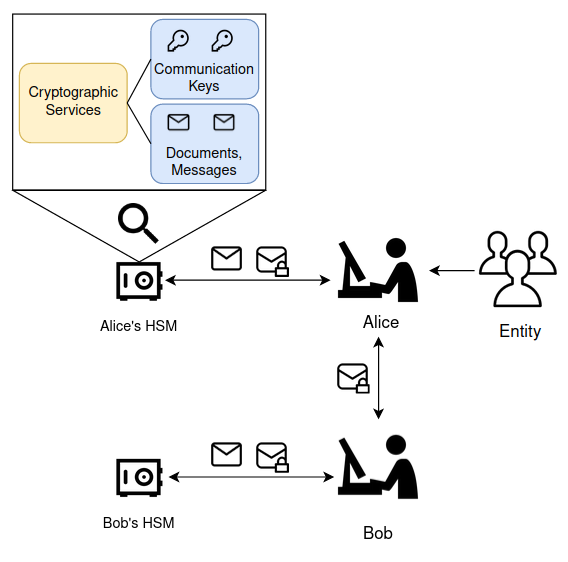
\includegraphics[width=0.75\textwidth]{./Images/overview2.png}
    \caption{System Overview}
    \label{fig:overview}
\end{figure}

%% SYSTEM OVERVIEW %%
The user's computer running the software is connected to the device, through a physical connection, used to send and receive data and commands.
Using these tools, the user can signal the device to perform the desired services.
These services are implemented inside the device, which stores and manages keys, as well as other data.
If the device is misplaced or stolen, the stored keys and documents are not at risk of being extracted. The developed software and physical tamper measures ensure it.
Upon receiving their device, each user is only required to connect it to their computer using the appropriate cable. The system is ready to use, through the provided interface software.

% -----------------------------------------------------
% -----------------------------------------------------
\section{Services}\label{chap:arch:services}

%% INTRODUCTION %%
This section describes each system service and all its relevant information. 
Firstly it presents the authentication, then the secure data exchange service, qualified digital signatures and services to establish new communication endpoints.

% -----------------------------------------------------
\subsection{Authentication}\label{chap:arch:services:auth}

Each entity will have its own device, which can be connected to a computer. To access the device's services, all users need to be authenticated to the device, through a PIN number. There is only a single PIN number, to authenticate the user's belonging to an entity to their device. This PIN number is securely stored in the device.
Each entity can supply this number to users which will use the device, in behalf of the entity.
After the user sends the correct PIN and is authenticated, the PIN can be changed.

% -----------------------------------------------------
\subsection{Secure Data Exchange}\label{chap:arch:services:data-exchange}

As previously introduced, the main goal of this solution is to secure communications between multiple entities, with identical devices.
Herein defined is the secure data exchange service, responsible for securing communications between entities. 
Communications are secured by providing three services: confidentiality, integrity and authentication. This allows communicating entities to ascertain the origin of messages and prevent unauthorized entities from reading and modifying them.
To grant these services, communicating entities must agree on a symmetric key. This key will be stored in the devices of both entities, and is never exposed outside to the outside.
This system provides services to agree on keys, which are discussed further ahead. For the purpose of this section, we will assume a symmetric key has already been agreed between both entities.

As discussed in the previous chapter, and depicted in Figure \ref{fig:overview}, Alice's computer will communicate with her HSM, in order to secure data, to be sent to Bob. For this, there needs to be a communications protocol between the computer and HSM, to define what data is sent, in what order and by who. To secure a piece of data sent by Alice, the device needs to receive the data, and return the data encrypted and authenticated with an internal key, previously agreed by Bob and Alice.
Thus, the communication protocol, between the device and computer application, is illustrated in Figure~\ref{fig:protocol:data-exchange}.
\begin{figure}[h!]
	\centering
	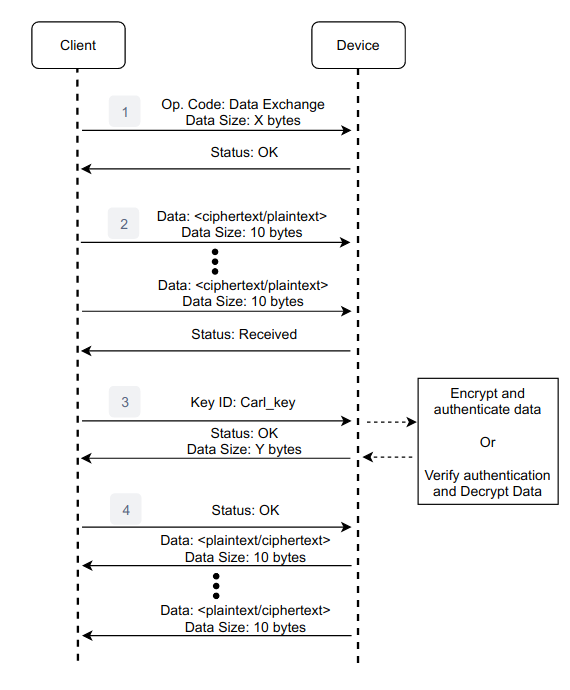
\includegraphics[width=0.60\textwidth]{./Images/data-exchange.png}
	\caption{Communication protocol for data ciphering and authentication in the HSM with internal keys}
	\label{fig:protocol:data-exchange}
\end{figure}
Since the system is designed to have multiple services, and be able to store multiple keys, there needs to be a mechanism to identify the different services and keys.
Services will be identified through a operation code, with a unique value for every service. Similarly, keys will be identified through an ID with a unique value for every key. Alice must know the ID for every key, which is stored in the device along with the corresponding key.

Thus, if Alice wants to secure data, the computer must first send a message composed of a 1 byte code, identifying the secure data exchange service, and a 1 byte key ID, to identify the symmetric key which will be used to secure data.
Upon receiving the message, the device will check internally if the user is authenticated and if both the operation code corresponds with an existing service and if the key with the corresponding ID exists.
Subsequently the corresponding success or failure status is returned by the device.

After a successful exchange, the data can be sent to the device. Before the data is received, the device must know the size of the data which it will receive from the computer. Thus, 2 bytes containing the data size are sent first.
After the data is processed in the device, its output is sent back to Alice, which can be securely sent to another entity, with the same symmetric key in their device.
If Bob wants to obtain the plaintext of the data sent by Alice, the same communication process is used. Bob sends the correct operation code and key ID, receives a success status response, then sends the secured data from Alice, and waits for the plaintext response. 

To produce the secure data, the plaintext must be encrypted and authenticated to provide the three necessary cryptography services: confidentiality, authentication and integrity.
On the other hand, there must also be a process to authenticate and decrypt the data, in order to retrieve the plaintext. Therefore, a protocol for encryption and encryption with authentication is needed.

As presented in Section \ref{chap:background:crypto}, symmetric encryption schemes provide confidentiality to data, while MAC algorithms provide authentication. AEAD schemes, which authenticate and encrypt messages, such as AES-GCM, may be more efficient and are less likely to be misused, than combining separate encryption and authentication schemes.
Unfortunately, devices such as the SmartFusion2 SoC, do not provide AEAD schemes. These boards usually provide separate encryption and authentication algorithms.
Thus, the proposed solution combines an encryption and authentication scheme, in order to provide the necessary cryptography services.
Both algorithms can be combined in different orders. Studies recommend combining a secure encryption and secure MAC, with the encrypt-then-MAC method~\cite{encryptmacorder}. This method encrypts the plaintext first, then generates the MAC from the generated ciphertext.

From this information, the proposed encryption protocol is pictured in Figure \ref{eq:encrypt-mac}. First, the plaintext data is encrypted with an internal symmetric key and a randomly generated IV. Next, a MAC is generated from the concatenated IV and ciphertext.
If the IV can be modified by an attacker, the original plaintext cannot be fully recoverable. Therefore, it is important that the MAC is generated from both the ciphertext and IV, this way the receiver can detect if either information was altered.
The output data is the concatenation of the IV, ciphertext and MAC.
\begin{equation}
	\label{eq:encrypt-mac}
	E_{key}\{Data, IV\}, MAC_{key}\{IV+E_{key}\{Data, IV\}\}
\end{equation}

The decryption protocol is pictured in Figure \ref{eq:decrypt-mac}. The protocol follows the same process as the previous but in reverse order. A new MAC is generated from the received IV and ciphertext. Then, the computed and received MACs are compared. If identical, the receiver can be sure of the data's origin and integrity. The ciphertext is decrypted with the same internal symmetric key used for encryption and the received IV, to obtain the plaintext.

\begin{equation}
	\label{eq:decrypt-mac}
	(MAC_{key}\{IV+Ciphertext\} == MAC) => E_{key}\{Ciphertext, IV\} => Data
\end{equation}

% ----------------------------------
\subsection{Qualified Digital Signatures}\label{chap:arch:services:signatures}

Digital signatures provide non-repudiation to a piece of data. This prevents an entity from denying the authorship of message. Qualified signatures are a special type of signatures where the private keys, which generated them, are stored inside a device, such as a HSM, and are never exposed to the outside.
Therefore, the signature must be generated inside the HSM. The device should support an algorithm for the generation of signature, such as ECDSA.
The device will store a unique private key, which will identify the entity. This key is randomly generated in the device and subsequently stored. Afterwards, the system is delivered to entities, with the already generated key.

As with the previous service, a communications protocol between the user and device must be defined. The device must receive the data, from which it will generate the signature, while the user will receive the generated signature.
The devised communication protocol is presented in Figure~\ref{fig:protocol:signature-generate}.
\begin{figure}[h!]
	\centering
	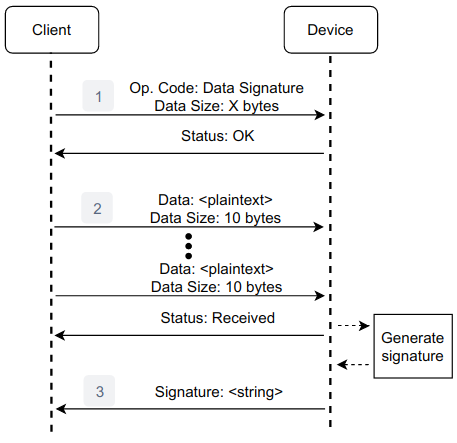
\includegraphics[width=0.55\textwidth]{./Images/signature-generate.png}
	\caption{Communication protocol for generating digital signatures using internal HSM asymmetric key pair}
	\label{fig:protocol:signature-generate}
\end{figure}
In order to identify the service, the user will send the corresponding operation code, along with the data to be signed.
Upon reception of the data, the device checks if the user is authenticated and subsequently generates the qualified signature, using its internal private key.
Afterwards, the device responds with the generated signature.

As discussed previously, public key cryptography is slow. Therefore, a digital signature is generated by first computing a hash of the message, then signing the hash with the private key, as shown in Figure \ref{eq:signature-generate}. In general, generating a signature from a hash is faster, since it has small fixed size, while the data can be of any size.

\begin{equation}
	\label{eq:signature-generate}
	Sign_{K}\{Hash\{Data\}\}
\end{equation}

% To verify a signatures, the user sends the operation code, signature length and generated signature, as well as the data length and data from which the signature was generated. The last piece of information sent is the public key of the device, where the signature was generated.
% After verifying the signature, the device responds with the operation status.
% The data is verified using the same hash function, ECDSA algorithm, and the signers' public key, as detailed in \ref{eq:signature-verify}.

% \begin{equation}
%         \label{eq:signature-verify}
%         \{Signature\} == Verify_{K_{-1}}\{Hash\{Data\}\}
% \end{equation}

% -----------------------------------------------------
\subsection{Establishing New Communication Endpoints}\label{chap:arch:services:new-comms}

The system provides the flexibility to establish secure communications with new entities, with identical devices.
To achieve this, entities must agree on a new symmetric key, which can be subsequently used with the secure data exchange service, presented in Section \ref{chap:arch:services:data-exchange}, to secure communications between them.
All new keys are stored in the device's secure storage, along with its unique ID.
Two different mechanisms to generate and agree on new symmetric keys are presented next. The first uses public key cryptography and the second uses symmetric key cryptography.

% -----------------------------------------------------
\subsubsection{Key Generation}\label{chap:arch:services:new-comms:ecdh}

The protocol to generate a shared symmetric key with another entity, using asymmetric cryptography is detailed in Figure~\ref{fig:protocol:ecdh}.
\begin{figure}[h!]
	\centering
	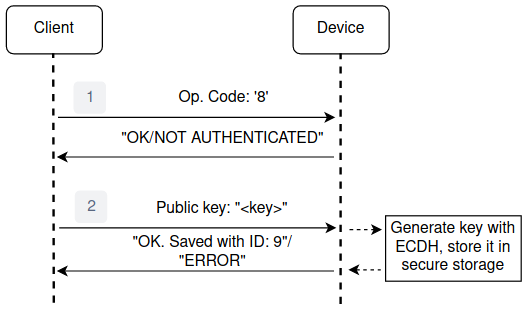
\includegraphics[width=0.60\textwidth]{./Images/ecdh.png}
	\caption{Communication protocol to generate symmetric keys, with an internal private key, to be stored internally}
	\label{fig:protocol:ecdh}
\end{figure}

% The user forwards the operation code, public key and salt value to the device.
The user forwards to the device, the operation code and the public information from the central station: the foreign entity's public key and an additional public salt component.
The generation process depicted in Figure \ref{fig:protocol:ecdh} is thus: first, a secret is computed with the ECDH algorithm, using the device's private key and the received public key. The secret is run through a key derivation function with the salt value, to obtain a new symmetric key.

\begin{equation}
	\label{eq:ecdh-kdf}
	KDF\{ECDH_{K}\{K^{-1}\}, Salt\}
\end{equation}

The same secret can be generated with the device's public key and the foreign entity's private key, in their device. If both entities receive each other's public keys and agree on the same salt value, through the central station, the generated key is identical.
A new unique ID is generated for the key, which is stored in the device, alongside the key. This ID is returned to the user, along with the operation status.
The salt value is used, in order to generate several symmetric keys from the same asymmetric key pairs.

% -----------------------------------------------------
\subsubsection{Import Keys}\label{chap:arch:services:new-comms:import}

This section details the protocol to import a list of encrypted symmetric keys into the device.
The imported keys must be encrypted with a preset symmetric key, stored inside the device from fabric, using the secure data exchange service. Thus, a central management section with a similar device can distribute keys to the enrolled entities, on a regular schedule.
The protocol for the service is depicted in Figure \ref{fig:protocol:import-keys}.

\begin{figure}[h!]
	\centering
	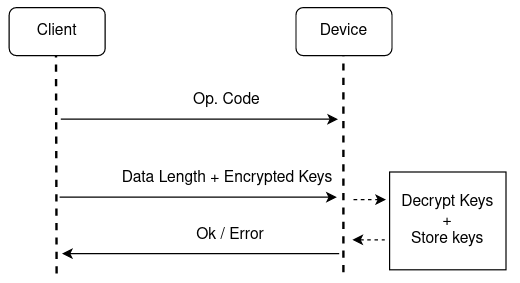
\includegraphics[width=0.60\textwidth]{./Images/import-keys.png}
	\caption{Communication protocol to import encrypted symmetric keys, and store them encrypted in the HSM's non-volatile memory}
	\label{fig:protocol:import-keys}
\end{figure}

The only transmission consists of sending the operation code, key set length and key data. Then, the device decrypts and authenticates the keys using a predefined symmetric key, stored in the device. The protocol used is the same for secure data exchange, as described previously.
Each key data section consists of 1 byte for its ID, 1 byte for its size and remaining bytes for the actual key data.
The decrypted list of keys is encrypted again, with a dedicated symmetric key for memory storage. 

The ciphertext and randomly generated IV are stored in memory. Both are authenticated by generating a MAC and storing it in secure storage.
In order to fetch a stored key, a MAC is generated from the ciphertext and IV in memory, and compared to the MAC in secure storage. If identical, the keys can be decrypted and a specific key identified through its ID.

% The device can also import a new set of keys, provided by the control station.
% This way, already established channels of communication can be updated on a regular time schedule.
% When a user wants to communicate with a new entity, the system provides two convenient solutions.
% Both options allow establishing connections with new entities when needed, by way of a trusted third party: a control station.
% The user can securely contact the control station at any time to request the public key of the other entity, through the secure data exchange service, equivalent to communicating with any other entity. The control station effectively acts as a PKI.
% Then, the user sends the information through the computer application to the device. The new key is generated in the device and made available right away. Then data can be exchanged with the new entity, which must also request the control station for the analogous entity's public key.

% The system can also be setup with a regular communication update schedule. It grants the flexibility of key revocation when needed, data exchange with new entities, as well as updating symmetric keys, with no additional complexity to the user, to always safeguard the security of communications.
% Each month an entity can hand over a list of the entities it wishes to communicate with to the control station, which will accordingly yield the corresponding key set.
% Each entity only needs to forward the list to the device, and the new keys are immediately stored and ready to be used.
% Users can resume communications, the same way as before with minimal interruption, with the requested entities.
% The protocols for both services are detailed next: symmetric key generation and importation of keys.

% -----------------------------------------------------
\section{Summary}\label{chap:arch:summary}

This section described the system's functionalities, algorithms and communications protocols, between a secure and portable device, and the user's computer application.
The system grants confidentiality and authentication to communications between any number of users, as soon as they receive the device, without overloading the users with convoluted tasks or responsibilities.
It is very flexible, by allowing entities to manage the authorized user's of their devices and with whom they wish to communicate, by offloading the management responsibility to a trusted control station.
